\documentclass[a4paper,12pt]{article}
\usepackage{graphicx}
\usepackage[utf8]{inputenc}
\usepackage[T1]{fontenc}
\usepackage[MeX]{polski}
\usepackage{titling}
\pagestyle{plain}
\title{Dokumentacja projektu Mrówka Langtona}
\author{Mikołaj Kubik 291083, Karol Stasiak 291107}
\date{\today}
\begin{document}
\begin{titlingpage}
\begin{center}
\begin{huge} 
\textbf{\thetitle}\\
\end{huge}
\vspace{0.2cm}
ver. 1.0 \\
\begin{center}
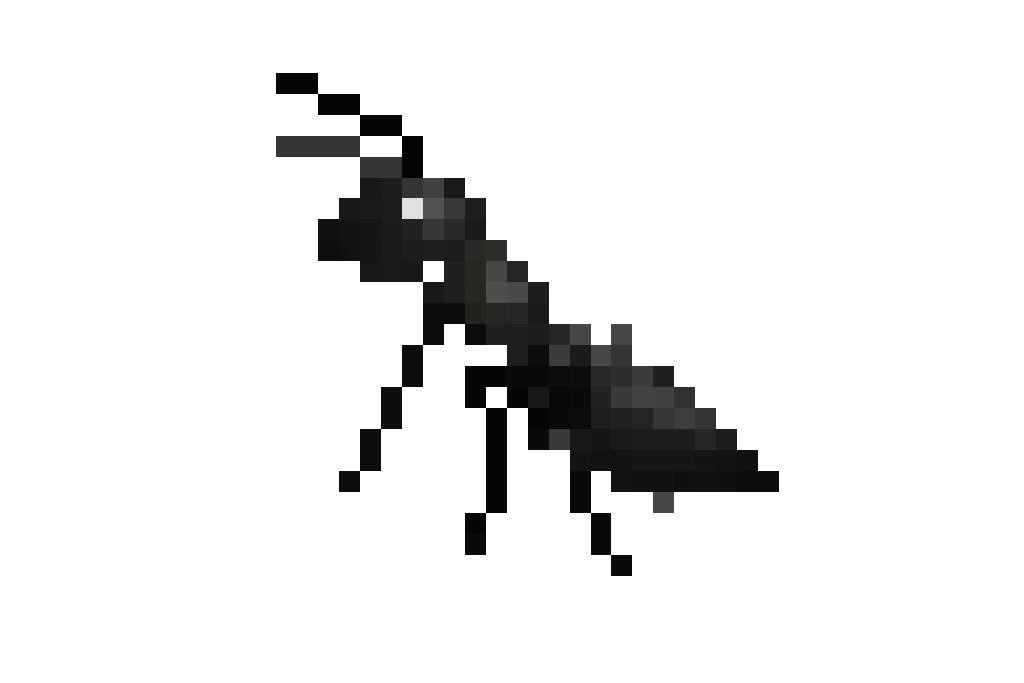
\includegraphics[height=3cm]{logo}
\end{center}
\vspace{0.2cm}
\theauthor\\
\vspace{0.2cm}
Grupa 15\\
\vspace{0.2cm}
\thedate\\
\vspace{0.5cm}
\begin{tabular}{|r|l|l|l|} \hline
wersja & zmiany & kto & kiedy \\
\hline
0.1 & Stworzenie dokumentu & KS & 21.03.2018 \\
\hline
0.2 & Edycja sekcji & MK & 02.04.2018 \\
\hline
0.3 & Edycja sekcji & KS & 03.04.2018 \\
\hline
1.0 & Zatwierdzenie dokumentu & MK & 03.04.2018 \\
\hline
\end{tabular} \\
\vspace{5,2cm}

\includegraphics[height=3cm]{ee}\\
\begin{large}
Politechnika Warszawska\\
Wydział Elektryczny\\
\end{large} 
\end{center}
\end{titlingpage}
\tableofcontents
\newpage
\section{Zasada działania mrówki}
\begin{enumerate}
\item Jeśli znajdzie się na polu białym to obraca się w lewo (o kąt prosty), zmienia kolor pola na swój kolor i przechodzi na następną komórkę;
\item Jeśli znajduje się na polu zakolorowanym to obraca się w prawo (o kąt prosty), zmienia kolor pola na biały i przechodzi na następną komórkę;
\item Porusza się na nieskończonej planszy podzielonej na kwadratowe komórki (zakolorowane lub nie), o rozmiarze 1 px każda;
\item Mrówki startują z wylosowanego miejsca na planszy;
\end{enumerate}
\section{Założenia projektu}
\begin{enumerate}
\item Program obrazuje symulację mrówki Langtona.
\item Program może zostać uruchomiony zarówno z ustawieniami domyślnymi, jak i podanymi przez użytkownika
\item Jeżeli użytkownik poda błędne argumenty, program zadziała zgodnie z argumentami domyślnymi dla danego parametru oraz wyświetli błąd.
\item Program może wyświetlić również animację ruchu mrówek w terminalu.
\item Użytkownik może podać dane zarówno z linii komend, jak i pliku tekstowego.
\item Maksymalne wymiary planszy wynoszą 10000 x 10000.
\item Program pozwala symulować zachowanie do 1000 mrówek.
\item Mrówki mogą wykonać maksymalnie 10000000 kroków.
\item Stan planszy po wykonaniu zadania zostaje zapisany do pliku png.
\item Po dojściu do skraju planszy mrówka automatycznie przechodzi na jej przeciwległy brzeg.
\item Początkowe współrzędne mrówek są ustawiane losowo.
%\item Początkowe współrzędne mrówek są pobierane z pliku, w przypadku podawania argumentów z pliku tekstowego.
\end{enumerate}
\section{Domyślne ustawienia}
\begin{itemize}
\item \textbf{Wymiary planszy:} 184 x 184
\item \textbf{Liczba mrówek:} 1
\item \textbf{Ilość kroków:} 11000
\item \textbf{Współrzędne początkowe:} Losowe
\item \textbf{Czy wyświetlić animację? :} 0 - nie
\item \textbf{Nazwa pliku png:} out.png
\end{itemize}
\section{Uruchamianie programu}
Argumenty dla programu (rozmiar planszy oraz liczba mrówek) mogą zostać podane zarówno z terminalu, jak i pliku tekstowego. Zastosowanie podanych wyżej przedrostków x (x to dany przedrostek) pozwoli na wpisywanie danych bez konieczności zachowania odpowiedniej kolejności.
\begin{itemize}
\item Nazwa wywoływanego programu \textbf{./ant}
\item Szerokość planszy \textbf{-w}
\item Wysokość planszy \textbf{-h}
\item Ilość mrówek \textbf{-q}
\item Ilość kroków \textbf{-n}
\item Czy wyświetlić animację w terminalu? (0 - nie, 1 - tak) \textbf{-a}
\item Nazwa pliku w którym ma zostać zapisany obraz \textbf{-o}
\item Nazwa pliku z danymi \textbf{-i}
\end{itemize}
\newpage
\subsection{W przypadku pliku tekstowego}
Po podaniu -i oraz nazwy pliku program wczyta potrzebne dane z pliku. Dane z pliku mają wyższy priorytet niż te wpisywane z konsoli. Jeżeli w pliku wystąpi jakiś błąd, dany argument zostanie zastąpiony domyślnym. Zachowanie kolejności przy wpisywaniu danych w pliku jest konieczne.
Argumenty muszą być oddzielone znakami nowej linii.
\textbf{Kolejność:}
\begin{enumerate}
\item Szerokość
\item Wysokość
\item Ilość mrówek
\item Ilość kroków
\item Czy wyświetlić animację? (0 - nie, 1- tak)
\item Nazwa pliku w którym ma zostać zapisany obraz
\end{enumerate}
\section{Obsługa błędów}
\begin{itemize}
\item Jeżeli wśród argumentów znajdzie się zmienna niebędąca liczbą, program przyjmie wartość domyślną dla danego argumentu oraz powiadomi o błędzie.
\item Jeżeli którykolwiek argument przekroczy zakres podany w założeniach, program zadziała zgodnie z ustawieniami domyślnymi dla tego argumentu oraz wyświetli odpowiedni komunikat.
\item Jeżeli liczba argumentów będzie zbyt duża, argumenty dodatkowe zostaną zignorowane.
%\item Jeżeli użytkownik poda pozycje startowe mrówek wykraczające poza planszę, program zakończy działanie oraz wyświetli informację o błędzie.
%\item Jeżeli ilość współrzędnych startowych nie będzie zgadzała się z ilością mrówek, mrówki zostaną rozmieszczone losowo.
\end{itemize}
\newpage
\section{Budowa programu}
Program podzieliliśmy na 5 części, aby ułatwić czytelność, modyfikacje oraz testy.
\begin{itemize}
\item \textbf{ant.c, ant.h} - odpowiada za implementację struktur ant\_t i ants\_t oraz sposobu poruszania się mrówek 
\begin{itemize}
\item struct* ant\_t
\item struct* ants\_t
\item void move(ant\_t, int)
\item void mirror(ant\_t, int ,int)
\item ants\_t ants\_init(int)
\item void free\_ants(ants\_t)
\end{itemize}
\item \textbf{matrix.c, matrix.h} - odpowiada za implementację struktury mat\_t, odpowiednią alokację pamięci na nią oraz opcjonalną animację mrówki w terminalu
\begin{itemize}
\item struct* mat\_t
\item mat\_t init(int, int)
\item void animate(mat\_t)
\item free\_matrix(mat\_t)
\end{itemize}
\item \textbf{exporttopng.c, exporttopng.h} - odpowiada za zapis planszy do pliku png
\begin{itemize}
\item void write\_png\_file(char*)
\item void process\_file(mat\_t)
\end{itemize} 
\item \textbf{error.c, error.h} - odpowiada za obsługę błędów
\begin{itemize}
\item checkMatrix(int x)
\item checkSteps(int x)
\item checkAmount(int x)
%\item checkHeight(int cord, mat\_t matrix)
%\item checkWidth(int cord, mat\_t matrix)
\end{itemize}
\item \textbf{main.c} - odpowiada za sterowanie programem. Działa jako reguła \textbf{main}.
\end{itemize}
Do programu dodatkowo załączyliśmy plik z regułą Makefile, mający na celu uproszczenie kompilacji oraz usuwania plików tymczasowych tworzonych przez program.
\section{Opis poszczególnych modułów}
\subsection{ant}
Struktura ant\_t zawiera 3 argumenty. Pierwsze dwa to współrzędne x oraz y odpowiadające za położenie mrówki na planszy. Trzeci argument informuje w którą stronę mrówka jest obecnie obrócona. Kolejna struktura ants\_t przechowuje mrówki z ant\_t oraz informacje o ich ilości. Funkcja move odpowiada za poruszanie się mrówki po planszy. Natomiast funkcja mirror obsługuje przypadek w którym mrówka natrafi na kraniec planszy, przenosząc ją na przeciwległy brzeg. W tym module inicjowana jest również struktura ants\_t oraz funkcja ją zwalniające free\_ants.
\subsection{matrix}
W module matrix tworzymy strukturę mat\_t zawierającą szerokość i wysokość macierz oraz tablicę t.
Następnie inicjujemy macierz. Funkcja animate odpowiada za wyświetlanie opcjonalnej animacji w terminalu. Natomiast funkcja free\_matrix która czyści strukturę mat\_t.
\subsection{exporttopng}
Moduł exporttopng implementuje dwie funkcje. process\_file tworzącą strukturę pliku png oraz write\_png\_file tworzącą sam plik.
\subsection{error}
W tym module zaimplementowane są funkcje sprawdzające zgodność danych wprowadzanych przez użytkownika. checkMatrix bada, czy macierz nie wykracza poza wartości maksymalne, checkSteps analogicznie analizuje liczbę kroków, a checkAmount liczbę mrówek.% checkHeight oraz checkWidth sprawdzają czy mrówka rozpoczyna swoją drogę na planszy. Jeżeli nie, jej miejsce startowe jest ustalane losowo.
\newpage
\section{Przykładowe wywołanie}
\textbf{Zastosowane zostały domyślne wartości}
\begin{center}

\includegraphics[height=10cm]{out}
\end{center}
\newpage
\section{Wywołanie z maksymalnymi argumentami}
\textbf{Należy pamiętać, że wartości maksymalne nie są ustalone przez rzeczywiste ograniczenia programu, a wygodę  i czytelność wyników. Otrzymanie symulacji obrazującej ustalone maksimum zajmuje około 10 minut.}
\begin{center}
\includegraphics[height=10cm]{maks}
\end{center}
\end{document}